\documentclass[12pt]{jsarticle}

\setcounter{secnumdepth}{3}
%\setcounter{figure}{1}
\usepackage[dvipdfmx]{graphicx}
\usepackage{amsmath}
\usepackage{float}

\pagestyle{myheadings}

\usepackage{titlesec}
\titleformat*{\section}{\large}
\titleformat*{\subsection}{\normalsize\bf}

\begin{document}

%{\LARGE レベル制御(PI制御)}
\section{目的}
 プロセス制御系の制御対象(プロセスまたはプラントともいう)は,一般に,炉,反応装置などの化学プロセスが主である.それらは分布定数系,もしくはむだ時間を含む系であることが多く,その応答時間は数分から数10分にもなり,サーボ系に比べ,極めてゆっくりとしているのが特徴である.ここでは,プロセス系の一つであるレベル制御を最も一般的なPID調節器の設計を通じて学習する.
\section{原理}
まず,図\ref{FigB1-1}に本実験で用いるレベル系のモデルを示す.ただし,図の記号は
\begin{flushleft}
  \setlength{\leftskip}{3.0cm}
     $u$:タンク1への流入量\\
     $q_i$:タンク$i$からの流出量($i$=1,2)\\
     $h_i$:タンク$i$の水位($i$=1,2)\\
     $A_i$:タンク$i$の断面積($i$=1,2)\\
     $R_i$:流体抵抗($i$=1,2)
\end{flushleft}
を意味する.
本実験では,タンク1への流入量$u$を入力とし,タンク2の水位$h_2$を出力とする制御対象の同定を行う.制御対象の伝達関数は
\begin{equation}
  \label{eqB1-1}
  \frac{H_2(s)}{U(s)} = \frac{R_2(s)}{(1+A_1R_1s)(1+A_2R_2s)}
\end{equation}
となり,対象とする系は二次遅れ系である.ただし,式(\ref{eqB1-1})の$U(s)$,$H_2(s)$は,それぞれ$u$および$h_2$のラプラス変換である.

\begin{figure}[H]
  \begin{center}
    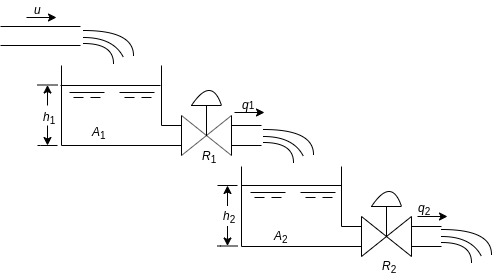
\includegraphics[clip,width=7.0cm]{../img/FigB1_1.png}
    \caption{レベル系}
    \label{FigB1-1}
  \end{center}
\end{figure}

\subsection{PID制御について}
PID制御の基本形を図\ref{PID-normal-form}に示す.スカラ制御系について説明する.すなわち,制御量,操作量,外乱の数をそれぞれ一とする.そうすると目標値から制御量を引いた値が偏差とみなせ,この偏差に基づいて操作量をいかに決定するかが問題となる.そこで,そのルール(制御則)を以下の三つについて考える.
\begin{description}
  \item[(1)] 偏差が小さければ操作量も小さくし,偏差が大きければそれに応じて大きくするのが妥当である.そこで,制御則に偏差に比例した項を含める.これを比例動作と呼び,P動作と略称する.
  \item[(2)] 自己平衡性をもつ制御対象に比例制御のみを行うと,目標値や外乱のステップ状の変化に対して最終的に一定の偏差が残ってしまう.これを定常偏差またはオフセットという.そこで,制御則に偏差の積分に比例した項を含めればこの定常偏差が除去できる.これを積分動作またはI動作と呼ぶ.
  \item[(3)] 偏差の増減の動向を操作量に反映すれば,より速く目標値に達することが期待できる.そこで,偏差の微分に比例する項も制御則に含める.これを微分動作またはD動作と呼ぶ.これは一種の予見動作である.
\end{description}
以上の動作を含む制御則がPID制御である.これを式で表すと次式のようになる.
\begin{equation}
  \label{}
  u(t) = K_p e(t) + K_I\int^t_0 e(\tau) d\tau + K_D \frac{de(t)}{dt}
\end{equation}
ここで,$u(t)$は操作量,$e(t)$は偏差,$K_P$,$K_I$,$K_D$は比例定数である.更にこれを変形して,
\begin{equation}
  \label{}
  u(t) = K_P\{ e(t) + \frac{1}{T_I}\int^t_0 e(\tau) d\tau + T_D\frac{de(t)}{dt}\}
\end{equation}
と表すのが慣例となっている.ここで,$K_P$を比例ゲイン,$T_I$を積分時間,$T_D$を微分時間と呼ぶ.PID制御系の設計は,これらの三つのパラメータの値を決めることであり,これをPID制御の調整(チューニング)という.この調整法は種々提案されており,そのなかで有名はZiegler-Nicholsの限界感度法である.
\begin{figure}[tb]
  \begin{center}
    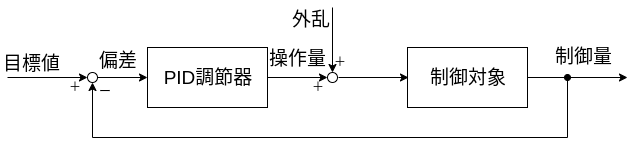
\includegraphics[clip,width=7.0cm]{../img/2-A1.png}
    \caption{PID制御系の基本形}
    \label{PID-normal-form}
  \end{center}
\end{figure}
\subsection{モデルの近似法}
プロセス制御系では,制御対象の特性は一般に非常に複雑で,物理的な考察から,伝達関数を正確に求めることができない場合が多い.しかし,そのステップ応答はS字型特性をもつことが多いので,むだ時間$L$を用いて近似し,伝達関数を
\begin{equation}
  \label{}
  G(s) = \frac{Ke^{-sL}}{Ts+1}
\end{equation}
と見なすことが多い.このように,一次遅れ+むだ時間系に近似すれば,わずか三つのパラメータで表せることになり,その取り扱いが簡単になる.\\
 一次遅れ+むだ時間系のステップ応答は,一次遅れ系のステップ応答をむだ時間$L$だけ時間軸上で遅らせた形で$t>L$に対して次のようになる.
\begin{equation}
  \label{}
  x(t) = \mathcal{L}^{-1}\left[\frac{Ke^{-sL}}{Ts+1}\frac{r}{s}\right] = rK(1 - e^{-\frac{t-L}{T}})
\end{equation}
複雑な系を一次遅れ系とむだ時間系の合成で近似しようとするとき,よく用いられる方法は,図\ref{LT_fromStepResponse}に示すように制御対象のステップ応答の変曲点Qで接線を引き,これを時間軸ならびに最終値との交点から$L$および$T$を決める方法である.
\begin{figure}[tb]
  \begin{center}
    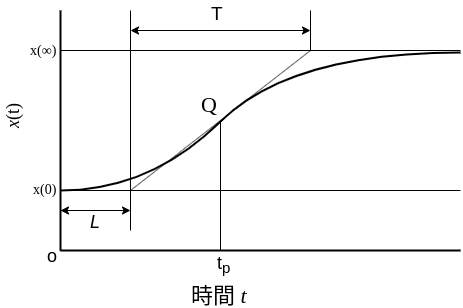
\includegraphics[clip,width=7.0cm]{../img/2-A2.png}
    \caption{ステップ応答から$L$と$T$を求める方法}
    \label{LT_fromStepResponse}
  \end{center}
\end{figure}

\subsection{限界感度法}
限界感度法は,制御対象の特性が一次遅れ+むだ時間系に近似できるとして,閉ループ系の過渡応答の行き過ぎ量が25\%程度となるように,PID調整器のパラメータを選ぼうとするものである.\\
 まず,図\ref{processController}の調整器をP動作のみとし,$K_P$を変化させて,閉ループ系が安定限界となる$K_P$の値を$K_C$とこのときの持続振動の周期$T_C$を求める.限界感度法は$K_C$と$T_C$をもとにして,パラメータ$K_P$,$T_I$,$T_D$を表のように求めるものである.\\
 この実験書では,調節器をPI動作として使用するので表\ref{Ziegler-Nichols}の→の箇所を使用すればよい.また,$K_C$と$T_C$は制御対象のボード線図(図\ref{Bode-Diagram})からも求めることができる.つまりそのゲイン余裕$g_m$[dB]と位相交点周波数(開ループ周波数特性の位相が-180[deg]となる周波数)$\omega_C$[rad/sec]より
\begin{eqnarray}
  \begin{cases}
    20{\rm log}_{10}K_C = g_m  [\rm dB] & \\
    T_C = \frac{2\pi}{\omega_C} [\rm sec] &
  \end{cases}
\end{eqnarray}
とすればよい.
\begin{table}[tb]
  \begin{center}
    \label{Ziegler-Nichols}
    \caption{Ziegler-Nicholsの限界感度法}
    \begin{tabular}{|c|c|c|c|} \hline
      $$ & $K_P$ & $T_P$ & $T_D$ \\ \hline \hline
      P動作   & $0.5K_C$  & $\infty$    & 0 \\ \hline
      →PI動作 & $0.45K_C$ & $0.83T_C$ & 0 \\ \hline
      PID動作 & $0.6K_C$  & $0.5T_C$  & $0.125T_C$ \\ \hline
    \end{tabular}
  \end{center}
\end{table}
\begin{figure}[tb]
  \begin{center}
    \label{processController}
    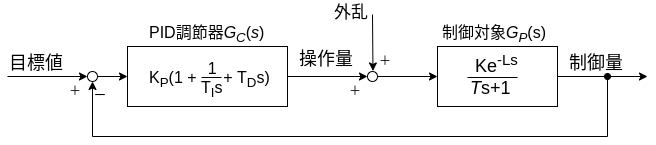
\includegraphics[clip,width=7.0cm]{../img/2-A3.png}
    \caption{プロセス制御系}
  \end{center}
\end{figure}
\begin{figure}[tb]
  \begin{center}
    \label{Bode-Diagram}
    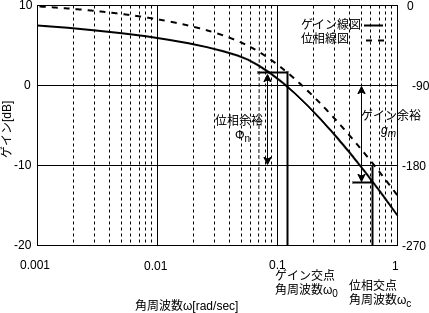
\includegraphics[clip, width=7.0cm, height=5.0cm]{../img/Fig2-A4.png}
    \caption{ボード線図}
  \end{center}
\end{figure}

\subsection{最小二乗法}
最小二乗法は,計測点が$X$のとき,$Y$と関数値$f(X)$との差$(Y-f(X))$を計算する.差の2乗$(Y-f(X))^2$が小さければ,$Y$と$f(X)$は近い値となる.差の2乗を全ての点で合計し,その合計値を最小にする.
\begin{equation}
  \label{minimum_required_method}
  T = \sum_{}^{}(Y-f(X))^2
\end{equation}
式(\ref{minimum_required_method})の$T$(合計)が最小となる関数の係数を求める.係数が求まると,任意の$X$での$f(X)$が求まる\cite{minimum_method}.
ここで,関数$y = a + bx_n$とすると,
\begin{eqnarray}
  \label{minimum_method}
  aN + b\sum_{n}^{}x_n = \sum_{n}^{}y_n \\
  a\sum_{n}^{}x_n + b\sum_{n}^{}x_n^2 = \sum_{n}^{}x_ny_n
\end{eqnarray}
となる.これを連立方程式としてとくと,
\begin{eqnarray}
a = \frac{\sum{}^{}y \sum{}^{}x^2 - \sum{}^{}xy\sum{}^{}x^2}{N\sum_{}^{}x^2 - (\sum_{}^{}x)^2}\\
b = \frac{N\sum{}^{}xy - \sum{}^{}x\sum{}^{}y}{N\sum_{}^{}x^2 - (\sum_{}^{}x)^2}
\end{eqnarray}
と求められる.

\section{実験装置と注意事項}
\subsection{実験装置}

まず,図\ref{FigB1-2}および表\ref{TableB1-2}にレベル実験装置の構成および装置の仕様をそれぞれ示す.計算機からD/A変換器を解して入力される電流値によって制御バルブMV1の開度が変化し,このバルブ開度に対応した流量の水がタンク1に入り手動バルブを介してタンク2に流入する.また,タンク2から制御バルブMV3を介して水が排出される.これら入出流量に依存するタンクの水位は差圧変換器によって計測され,D/A変換器を介して計算機に伝送される.特に,制御弁への制御電流と弁の開閉度との関係は4[mA]で全閉,20[mA]で全開となることに注意せよ.また,レベル実験装置には絶対に触らないこと(特にバルブなどに触れるとパラメータが変わる).
\begin{table}[tb]
  \label{TableB1-1}
  \caption{expappにおける表示の意味}
  %TODO
  \begin{tabular}{c|c|c} \hline
    表記 & 意味 & 備考\\ \hline \hline
    MV1 & タンク1注水用電磁バルブ指令電流値 & 4[mA]から20[mA] \\ \hline
    MV2 & タンク2注水用電磁バルブ指令電流値 & 4[mA]から20[mA] \\ \hline
    MV3 & 第二タンク排水用電磁バルブ指令電流値 & 4[mA]から20[mA] \\ \hline
    SAMPLING & サンプリング時間 & 1[s]から3[s]まで三段階で設定可能 \\ \hline
    APPLY & 設定値の変更を適用 & \\ \hline
    SV*[mA] & 電磁バルブ指令電流の設定値 & 実験前に表示 \\ \hline
    PV*[mA] & 電磁バルブ指令電流の現在地 & 実験中に表示 \\ \hline
    *[L/min] & 流量値 & \\ \hline
    *[V] & 差圧変換器出力 & \\ \hline
    IN & 入水経路 & \\ \hline
    OUT & 排水経路 & \\ \hline
  \end{tabular}
\end{table}
\begin{table}[tb]
  \label{TableB1-2}
  \caption{装置の仕様}
  \begin{tabular}{c|c|c} \hline
    装置 & 数 & 仕様\\ \hline \hline
    タンク1 & 1 & 高さ 1000[mm],内径 200[mm] \\ \hline
    タンク2 & 1 & 高さ 1500[mm],内径 320[mm] \\ \hline
    電流比例制御弁 & 3 &
    \begin{tabular}{c}
    弁開度入力信号:4~20[mA],全開-全閉時間:17[sec]以下,\\電源:24[VDC]±10\%
    \end{tabular} \\ \hline
    流量計 & 3 & オープンコレクタ出力,0.1[L/pulse] \\ \hline
    差圧変換器 & 2 & 容量:200[gf/c${\rm m^2}$] \\ \hline
    A/D変換ボード & 1 & 入力:8CH,0~10[V],分解能:12[bit],変換速度:10[sec/CH] \\ \hline
    D/A変換ボード & 1 & 出力:4CH,24[bit] up/down counter,変換速度:10[sec/CH] \\ \hline
    パスカルカウンタボード & 1 & 4CH,24[bit] up/down counter,外部入力:非絶縁TTL入力 \\ \hline
    コンピュータ & 1 & NEC PC9801RX \\ \hline
  \end{tabular}
\end{table}
\begin{figure}[tb]
  \begin{center}
    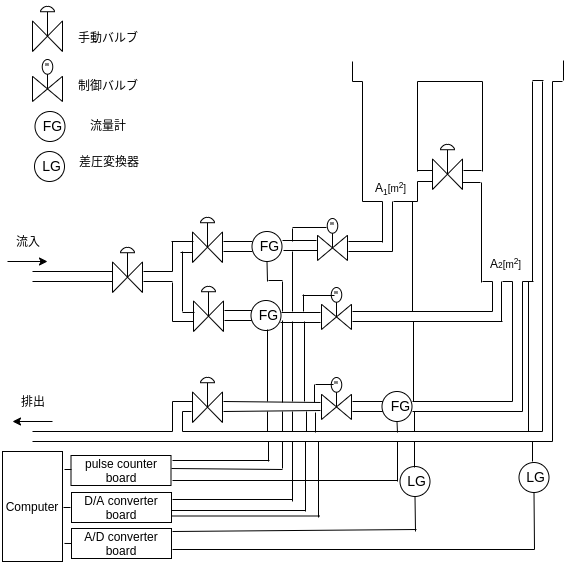
\includegraphics[clip,width=7.0cm]{../img/fig4.png}
    \caption{実験装置の構成}
    \label{FigB1-2}
  \end{center}
\end{figure}
\subsection{プログラム}
本実験で使用するプログラムは,USR3のホームディレクトリにあるexp3に下記の三種類のプログラムが格納されている.

\begin{description}
  \item[expapp:]制御弁特性の検証実験,差圧変換器特性の検証実験,流量の調整,タンク2水抜きのためのプログラム
  \item[step:]開ループ実験用プログラム
  \item[PID:]閉ループ実験用プログラム
\end{description}

これらのプログラムを実行するために,\\
cd exp3\\
としてディレクトリexp3に移動する.
\subsection{実験の開始時と終了時の操作}
実験の開始時の操作は必ず次の順序で行うこと.

\begin{description}
  \item[(1)] 配電盤のスイッチを入れる.
  \item[(2)] コンピュータの電源を入れる.
  \item[(3)] 元バルブを開く.
  \item[(4)] ./expappを実行し,制御弁を全開(20[mA])にして,流量が30[L/min]になるようにバルブ$V_1$を調整する.
\end{description}

また終了時には,これらを逆の順序で実行する.

\section{開ループ実験}
\subsection{実験(1) 制御弁}
流量の制御装置として使用している制御弁の動特性を調べた.
\begin{center}
  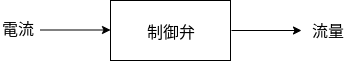
\includegraphics[clip,width=7.0cm]{../img/A_Q_transform.png}
\end{center}
プログラム「./expapp」を起動した.制御電流を4[mA]から20[mA]まで変化させ,そのときの定常状態の流量を測定し,電流-流量特性を求めた.
\subsection{実験(2) 差圧変換器(下段タンク用)}
水位検出器として使用している差圧変換器の動特性を調べた.
\begin{center}
  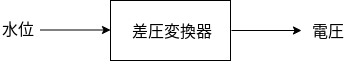
\includegraphics[clip,width=7.0cm]{../img/H_V_transform.png}
\end{center}
プログラム「./expapp」を起動した.制御弁を開閉して,タンク2の水位を増加させながら,そのときの差圧変換器の出力電圧を調べた.タンク2水位-出力電圧特性を求めた.ただし,測定する水位の上限は60[cm]とする.
\subsection{実験(3) 開ループ応答}
制御対象であるタンク1およびタンク2にステップ入力を加え,その過渡応答を求めた.
\begin{center}
  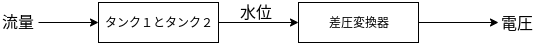
\includegraphics[clip,width=7.0cm]{../img/OpenResponse.png}
\end{center}
プログラム「./step」を起動した.プログラムの指示に従い,(1)制御弁の初期値,(2)変化量,(3)サンプリング周期を入力した.その後,[APPLY AND START]をクリックして実験を開始した.
まず,制御弁が初期位置まで開き,タンク1に水が流れ込む.タンク2の水位が定常地に収束した後に,[Recording Start]をクリックするとタンク2の差圧変換器の出力の計測が始まる.[Recording Start]をクリックしてから10サンプル時刻後に「変化量」で与えた値だけ更に制御弁が開き,タンク2の差圧変換器出力の計測が始まる.出力値が定常状態に収束したら「STOP」をクリックした.この時,ファイルネーム(英数字)に拡張子(dat)を付けて「SAVE ONLY」をクリックしてデータを保存した.データの横軸を時間軸に変換するには,「サンプル番号×サンプリング周期」とすればよい.
\subsection{モデル同定(第2週)}
各制御要素を次の手順で近似せよ.
\begin{itemize}
\item 実験(1)で電流-流量特性を作図するとともに,作動点近傍で線形化し制御弁のゲインを求め,ブロック線図を描け.
\item 実験(2)で下段タンク水位-出力電圧特性を作図するとともに,線形化し差圧変換器のゲイン(必要ならオフセットも)を求め,ブロック線図を描け.更に,次週で使用するので,出力電圧-水位の関係も求めておくこと.
\item 実験(3)で得られた結果を作図し,タンク1およびタンク2の伝達関数を一次遅れ+むだ時間で近似し,ブロック線図を描け.
\item 実験(1)-(3)で決定した各要素の合成結果と実験結果とを比較検討せよ.
\end{itemize}
\subsection{PID調節器の調整}
開ループの結果より,Ziegler-Nicholsの限界感度法に基づきPID調節器のパラメータを決定した.なお,限界感度法においてはBode線図を作図して決定すること.本実験では,PI動作のみで制御を行った.つまり,PID調節器のパラメータ$T_D$とし他の$K_P$と$T_I$を調整する.
\begin{figure}[tb]
  \begin{center}
    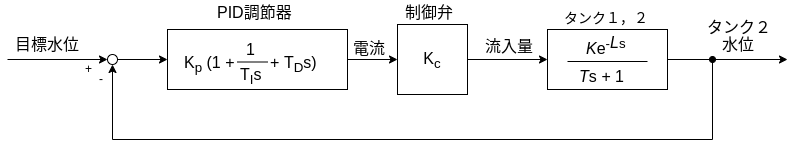
\includegraphics[clip,width=7.0cm]{../img/PIDController.png}
    \caption{フィードバック制御系}
    \label{FeedbackController}
  \end{center}
\end{figure}
\subsection{閉ループ実験(第3週)}
プログラム「./PID」を起動した.
プログラムの指示に従い,以下のパラメータを入力した.\\
(1)比例ゲイン,(2)積分時間,(3)微分時間,(4)タンク2の目標水位,(5)差圧変換器のゲイン$D_{gain}$及びオフセット$D_{offset}$,(6)サンプリング周期\\
ここで,差圧変換器の出力$D_{out}$[V]と水位$H$[cm]の関係を
\begin{equation}
  D_{out} = H・D_{gain} + D_{offset}
\end{equation}
として計算している.目標水位は40[cm]とした.\\
 [APPLY AND START]をクリックして実験を開始した.[Apply disturbance]をクリックすると,外乱要素として排水用制御弁の開度が変化するので,その応答を観測し検討した.600サンプル後もしくは[STOP]ボタンをクリックした後,[SAVE OK]をクリックしてデータを保存し,ファイルネーム(英数字)に拡張子(.dat)を付けて保存した.

\section{実験結果}
\subsection{開ループ実験の実験結果}

実験で得られた結果を表\ref{Table-I-Q},図\ref{Fig-I-Q},表\ref{Table-H-V},図\ref{Fig-H-V}に示す.
\begin{table}[htbp]
  \begin{center}
    \label{Table-I-Q}
    \caption{流量とバルブの特性}
    \begin{tabular}{|c|c|} \hline
    電流[mA] & 流量[L/min] \\ \hline \hline
     4.0 &  0.0 \\ \hline
     5.0 &  0.0 \\ \hline
     6.0 &  0.0 \\ \hline
     7.0 &  7.2 \\ \hline
     7.2 &  8.4 \\ \hline
     7.4 & 10.8 \\ \hline
     7.6 & 12.0 \\ \hline
     7.8 & 14.4 \\ \hline
     8.0 & 15.6 \\ \hline
     8.2 & 16.8 \\ \hline
     8.4 & 19.2 \\ \hline
     8.6 & 20.4 \\ \hline
     8.8 & 21.6 \\ \hline
     9.0 & 21.6 \\ \hline
    10.0 & 24.0 \\ \hline
    11.0 & 27.6 \\ \hline
    12.0 & 27.6 \\ \hline
    13.0 & 28.8 \\ \hline
    14.0 & 27.6 \\ \hline
    15.0 & 28.8 \\ \hline
    16.0 & 28.8 \\ \hline
    17.0 & 28.8 \\ \hline
    18.0 & 28.8 \\ \hline
    19.0 & 28.8 \\ \hline
    20.0 & 28.8 \\ \hline
    \end{tabular}
  \end{center}
\end{table}
\begin{figure}[tb]
  \begin{center}
    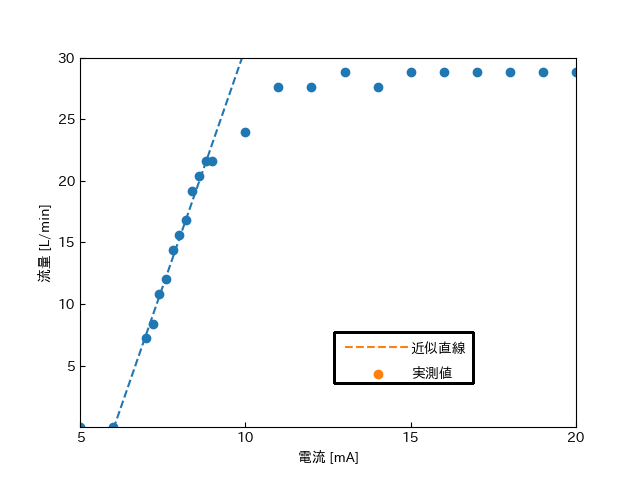
\includegraphics[clip,width=7.0cm]{../graph/approximity_IQ.png}
    \caption{流量とバルブの特性}
    \label{Fig-I-Q}
  \end{center}
\end{figure}
\begin{table}[htbp]
  \begin{center}
    \label{Table-H-V}
    \caption{差圧変換器の特性}
    \begin{tabular}{|c|c|} \hline
      水位[cm] & 電圧[V] \\ \hline \hline
       5.01 & 0.325 \\ \hline
      10.09 & 0.867 \\ \hline
      14.92 & 1.370 \\ \hline
      20.40 & 1.951 \\ \hline
      24.95 & 2.440 \\ \hline
      29.85 & 2.967 \\ \hline
      34.79 & 3.495 \\ \hline
      39.83 & 4.032 \\ \hline
      44.86 & 4.569 \\ \hline
      49.71 & 5.087 \\ \hline
      55.09 & 5.668 \\ \hline
    \end{tabular}
  \end{center}
\end{table}
\begin{figure}[tb]
  \begin{center}
    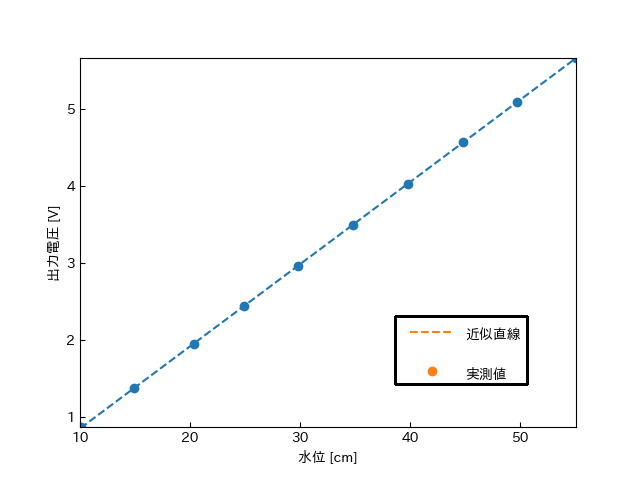
\includegraphics[clip,width=7.0cm]{../graph/approximity_HV.png}
    \caption{差圧変換器の特性}
    \label{Fig-H-V}
  \end{center}
\end{figure}
最小二乗法を用いて線形化を行うと次の二つの式が得られる.
\begin{equation}
  \label{}
  v(t) = 0.1067h(t) - 0.217
\end{equation}

\begin{equation}
  q(t) = 7.745i(t) - 46.691
\end{equation}
ブロック線図を描くと,それぞれ図\ref{BlockDiagIQ},図\ref{BlockDiagVH}になる.
\begin{figure}[tb]
  \begin{center}
    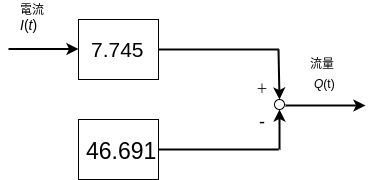
\includegraphics[clip,width=7.0cm]{../img/BlockDiagIQ.png}
    \caption{電流-流量特性のブロック線図}
    \label{BlockDiagIQ}
  \end{center}
\end{figure}
\begin{figure}[tb]
  \begin{center}
    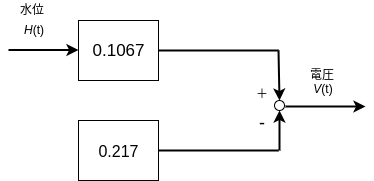
\includegraphics[clip,width=7.0cm]{../img/BlockDiagHV.png}
    \caption{出力電圧-水位特性のブロック線図}
    \label{BlockDiagVH}
  \end{center}
\end{figure}

ステップ応答の流量の結果を図\ref{Result-StepResponse-Q}に,差圧変換器出力電圧の結果を図\ref{Result-StepResponse-V}に示す.
\begin{figure}[tb]
  \begin{center}
    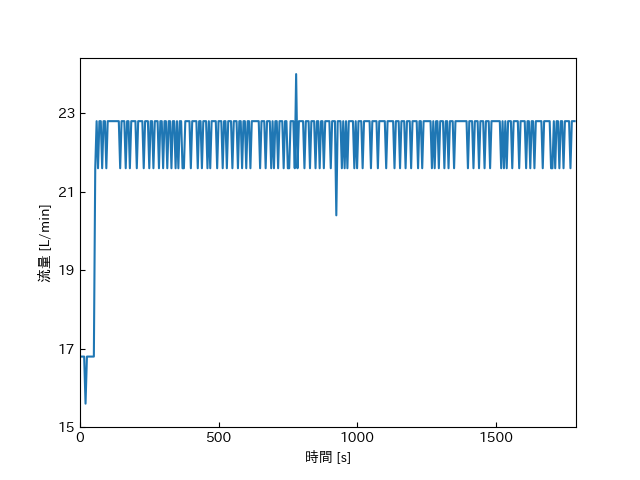
\includegraphics[clip,width=7.0cm]{../graph/StepResponseQ.png}
    \caption{ステップ応答の流量}
    \label{Result-StepResponse-Q}
  \end{center}
\end{figure}
\begin{figure}[tb]
  \begin{center}
    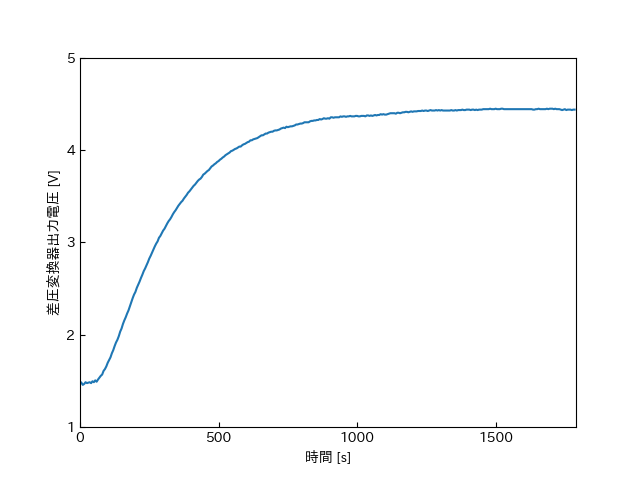
\includegraphics[clip,width=7.0cm]{../graph/StepResponseV.png}
    \caption{ステップ応答の電圧}
    \label{Result-StepResponse-V}
  \end{center}
\end{figure}

\subsection{モデル同定(第2週)の結果}
ステップ応答の出力に補助線を引き,$T$,$L$を求める.

また,ステップ入力のゲイン及び伝達関数のゲインは
\begin{eqnarray}
  \label{}
  r &=& Q(\infty) - Q(0) \\
  &=& 6.0
\end{eqnarray}
\begin{eqnarray}
  \label{}
  k &=& \frac{H(\infty) - H(0)}{r} \\
  &=& 4.61574
\end{eqnarray}
である.
よって,
\begin{equation}
  \label{}
  rk = 27.6944
\end{equation}

よって,伝達関数は次のようになる.
\begin{equation}
  \label{}
  G(s) = \frac{4.616}{370s+1}e^{-75s}
\end{equation}
これをブロック線図で描くと,図\ref{Tank_BlockDiag}となる.
\begin{figure}[tb]
  \begin{center}
    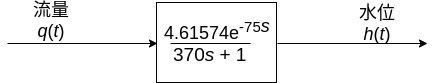
\includegraphics[clip,width=7.0cm]{../img/Tank_BlockDiag.png}
    \caption{タンク1,2のブロック線図}
    \label{Tank_BlockDiag}
  \end{center}
\end{figure}
ここでステップ応答$U(s)=\frac{r}{s}$を加えた結果を図\ref{StepResponseModeling}に示す.
ボード線図を描くことを考える.
\begin{figure}[tb]
  \begin{center}
    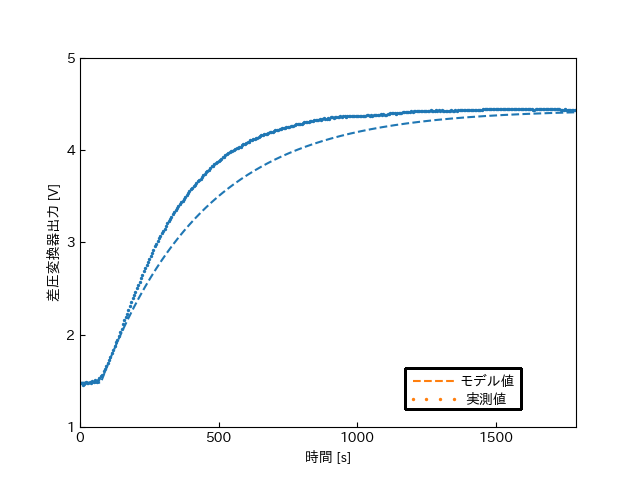
\includegraphics[clip,width=7.0cm]{../graph/stepResponse_approximity.png}
    \caption{ステップ応答のモデル化}
    \label{StepResponseModeling}
  \end{center}
\end{figure}
相対誤差は次式により求めることができる.
\begin{equation}
  E = \frac{|v(t) - v^{\prime}(t)|}{v^{\prime}(t)}
\end{equation}
ここで,$v^{\prime}(t)$は伝達関数のステップ応答の結果とする.
相対誤差の平均値は$4.9\%$であった.
\begin{eqnarray}
  20{\rm log}|G(j\omega)| &=& 20{\rm log}|\frac{4.616}{370j\omega+1}| + 20{\rm log}|e^{-75j\omega}| \\
  &=& 20{\rm log}\frac{4.616}{\sqrt{370^2\omega^2+1}} + 20{\rm log}1 \\
  &=& 20{\rm log}\frac{4.616}{\sqrt{370^2\omega^2+1}}
\end{eqnarray}
\begin{eqnarray}
  \angle G(j\omega) &=& \angle \frac{4.616}{370j\omega+1} + \angle e^{-75j\omega} \\
  &=& {\rm tan}^{-1}370\omega - 75\omega
\end{eqnarray}
そのため,ボード線図は図\ref{BodeDiagram}となる.

\begin{figure}[tb]
  \begin{center}
    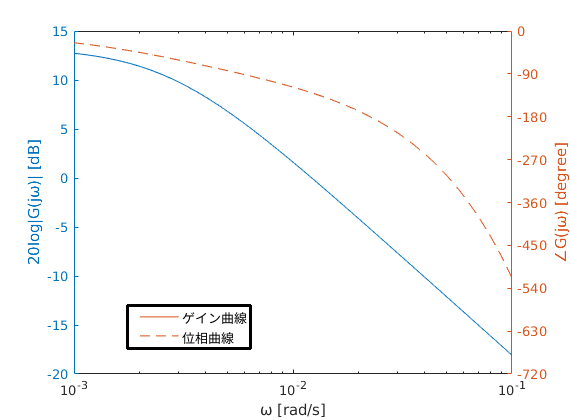
\includegraphics[clip,width=7.0cm]{../graph/BodeDiagram.png}
    \caption{ボード線図}
    \label{BodeDiagram}
  \end{center}
\end{figure}

この伝達関数のステップ応答を求める.
\begin{equation}
  \label{}
  v(t) = rk(1 - e^{-(t - 75)/370}) + v(0)
\end{equation}
実験結果との相対誤差を求めると,$\%$であった.

よって,ゲイン余裕,位相余裕,ゲイン交点周波数,位相交点周波数は次のようになる.
$G_m=5.19993$,$P_m=50.189$,$W_{cg}=0.0225354$,$W_{cp}=0.0121766$ \\
これらより,$K_C$,$T_C$を求めると,
\begin{eqnarray}
  \label{}
  K_C &=& 10^{\frac{g_m}{20}} \\
  &=& 1.81968
\end{eqnarray}
\begin{eqnarray}
  \label{}
  T_C &=& \frac{2\pi}{\omega_C} \\
  &=& 278.8057
\end{eqnarray}
これより,Ziegler-Nicholsの限界感度法を用いると,
\begin{eqnarray}
  \label{}
  K_P &=& 0.45 K_C \\
  &=& 0.818
\end{eqnarray}
\begin{eqnarray}
  T_I &=& 0.83 T_C \\
  &=& 231.4
\end{eqnarray}

\subsection{閉ループ実験(第3週)の結果}
(1)比例ゲイン,(2)積分時間,(3)微分時間,(4)タンク2の目標水位,(5)差圧変換器のゲイン$D_{gain}$及びオフセット$D_{offset}$,(6)サンプリング周期をそれぞれ,0.818,231.4,0,40,0.106,-0.217,1としてプログラムを実行した.
その結果を図\ref{PIDExp}に示す.
\begin{figure}[tb]
  \begin{center}
    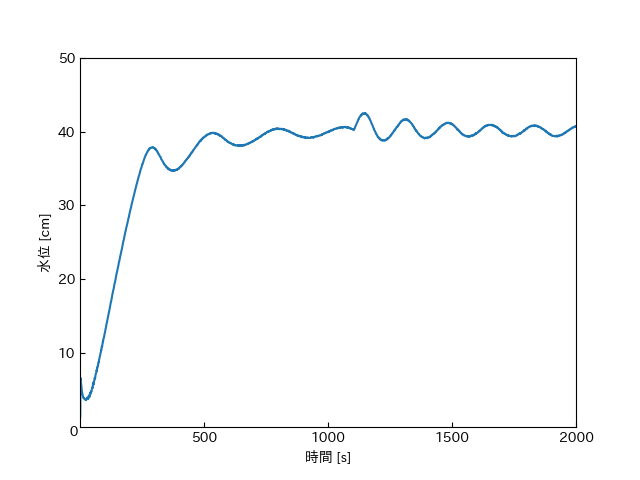
\includegraphics[clip,width=7.0cm]{../graph/PID_controll.png}
    \caption{PID制御実験の結果}
    \label{PIDExp}
  \end{center}
\end{figure}
\section{考察}
即応性を上げることについて考える.
$K_P$,$T_I$,$T_D$について,まとめる\ref{bibitemPID_Base_and_Ouyou}.
\begin{description}
\item[(1)] 比例ゲイン
  $K_P$だけを上げていくと:
  \begin{description}
  \item[I] オフセットは減少する.
  \item[II] 応答曲線の周期が短くなる.
  \item[III] $K_P$を上げすぎると不安定になる.
  \end{description}
\item[(2)] 積分動作
  $T_I$だけを小さくしていくと:
  \begin{description}
  \item[I] オフセットはなくなる.
  \item[II] 設定値への回復速度が速くなる.
  \item[III] $T_I$を小さくしすぎると不安定になる.
  \end{description}
\item[(3)] 微分動作
  $T_D$だけを大きくしていくと:
  \begin{description}
  \item[I] 安定度がよくなる.
  \item[II] 振動周期が短くなる.
  \end{description}
\end{description}
よって,即応性を上げるためには$K_P$を大きくし,$T_I$を小さくし,$T_D$を大きくすることが必要である.
\section{課題}
\begin{description}
\item[(1)]結果をグラフに描き,応答を考察せよ.\\ %TODO
\item[(2)]PI調節器+制御対象のボード線図を描き,ゲイン余裕と位相余裕を考察せよ.\\
開ループ伝達関数は次式のようになる.
\begin{eqnarray}
  \label{PID_openG}
  G_o(s) &=& \{K_P(1+\frac{1}{T_Is})\}\{\frac{Ke^{-Ls}}{1+Ts}\} \\
  &=& \{0.818(1+\frac{1}{231.4s})\}\{\frac{4.61574e^{-75s}}{1+370s}\}
\end{eqnarray}
これよりボード線図は図\ref{BodeChart_PID}となる.
\begin{figure}[tb]
  \begin{center}
    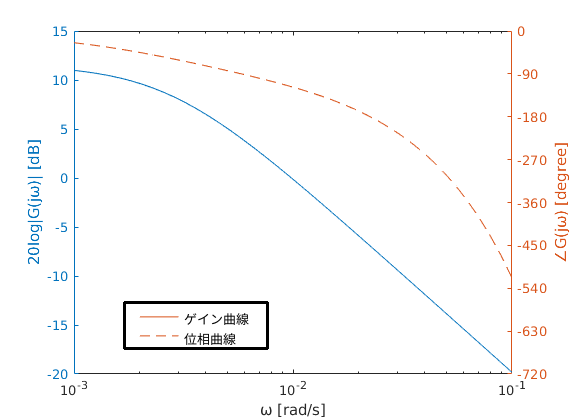
\includegraphics[clip,width=7.0cm]{../graph/BodeChart_PID.png}
    \caption{PI調節器+制御対象のボード線図}
    \label{BodeChart_PID}
  \end{center}
\end{figure}
よって,位相余裕は$63.0735°$,ゲイン余裕は$2.2242[dB]$となった.
位相余裕とゲイン余裕は,小さすぎると安定度が悪くなるし,大きすぎると速応性が悪くなる.経験的には,サーボ系では,位相余裕は40°〜60°.ゲイン余裕は10[dB]〜20[dB].プロセス制御系では,位相余裕は20°以上,ゲイン余裕は3[dB]〜10[dB]が良いとされている\ref{bibitemFundamentalAutonomaticControl}.
今回の制御対象はプロセス系であるため,概ね満足していると考えられる.
\item[(3)]PID調節器のパラメータの決め方は,他にどんなものがあるのか調べよ.\\
パラメータの設計法には,限界感度法やステップ応答法など試行錯誤的に設計する方法,周波数特性(位相・ゲイン余裕)に基づいて設計する方法,規範モデリングとのマッチングにより設計する方法,などが挙げられる.\\
まず,制御対象の数学モデルを用いて系統的に設計を行うモデルマッチング法を説明する.モデルマッチングにより設計するためには,制御対象の数学モデルが必要である.系の数学モデルが式\ref{modelMatching-transform}で与えられたとき,モデルマッチング法は,図\ref{modelMatching-Fig}に示すように,ある適切な規範モデル$M(s)$を与え,それに目標値$r(s)$から制御量$y(s)$までの伝達関数$g(s)$を一致させる(または近づける)というものである.つまり,望ましい制御系の極を実現するように極配置を行うということである.\\
\begin{equation}
  \label{modelMatching-transform}
  Y(s) = \frac{K}{1+Ts}U(s)
\end{equation}
規範モデルとしては,二項係数標準形やButterworth標準形がよく利用される.たとえば,2次系の規範モデル
\begin{equation}
  \label{modelMatching-teachmodel}
  M(s) = M_2(s) := \frac{\omega_n^2}{s^2 + 2\zeta \omega_ns + \omega^2}
\end{equation}
において,減衰性に関するパラメータ$\zeta$を$\zeta=1$と選んだものが二項係数標準形であり,$\zeta=1/\sqrt{2}$としたものがButterworth標準形である\ref{bibitemPendulum}.\\
 つぎに,CHR法を示す.Chien,Hrones and Reswickにより提案された方法である.これはこの3名の頭文字をとってCHR法と言われる.設定値変更及び外乱に対して,それぞれ「オーバーシュートなし」,および「オーバーシュート20\%」になるようなパラメータを求めている.表\ref{CHR-tuning}にそれを示す\ref{bibitem}.
\begin{table}[tb]
  \begin{center}
    \label{CHR-tuning}
    \caption{CHR法によるチューニング方法}
    \begin{tabular}{|c|c|c|c|c|c|} \hline
      制御目標 & 制御モード & 比例ゲイン$K・K_P$ & 積分時間$T_I$ & 微分時間$T_D$ & オーバーシュート \\ \hline \hline
       & P & $0.3T/L$ & - & - & \\
       & PI & $0.35T/L$ & $1.2T$ & - & なし\\
       設定値 & PID & $0.6T/L$ & $T$ & $0.5L$ &\\ \cline{2-6}
       変更 & P & $0.7T/L$ & - & - & \\
       & PI & $0.6T/L$ & $T$ & - & $20\%$\\
       & PID & $0.95T/L$ & $1.35T$ & $0.47L$ &\\ \hline
       & P & $0.3T/L$ & - & - & \\
       & PI & $0.6T/L$ & $4T$ & - & なし\\
       外 & PID & $0.95T/L$ & $2.4T$ & $0.4L$ &\\ \cline{2-6}
       乱 & P & $0.7T/L$ & - & - & \\
       & PI & $0.7T/L$ & $2.3L$ & - & $20\%$\\
       & PID & $1.2T/L$ & $2L$ & $0.42L$ &\\ \hline
    \end{tabular}
  \end{center}
\end{table}
\end{description}

\section{まとめ}
PID制御に使用するPID調節器の設計を習得した.

\begin{thebibliography}{9}
  \bibitem{minimum_method} 神足史人,Excelで操る!ここまでできる科学技術計算,p36,p37,2018.
  \bibitem{bibitemPendulum} 川田昌克ら,倒立振子で学ぶ制御工学,p26-29,2017.
  \bibitem{bibitemPID_Base_and_Ouyou} 川本重彦ら,PID制御の基礎と応用,p89,p92,1997.
  \bibitem{bibitemFundamentalAutonomaticControl} 鈴木隆ら,例題で学ぶ自動制御の基礎,p116,2011.
\end{thebibliography}

\end{document}
